% Joint-parameter stress test of the calibrated claims (round 3; author decision 7 of 2 November, 23:23).
% Method: notes/mc_claims_method.md; results: notes/mc_results_2026-11-03/mc_claims_report.md and seed2/ (code/mc_claims.py).
% Every number is a macro of paper1/stress_macros.tex (code/mc_report_tex.py) or of paper1/macros.tex.
\clearpage
\section{A joint-parameter stress test of the calibrated claims}\label{supp:stress}
\emph{Method.} Section~\ref{sec:horizons} of the main paper moves its calibrated inputs one at a time (Table~\ref{tab:tornado}) and through named bounds. This section moves them together, over the ranges the paper itself states, and asks of each headline claim whether it holds at every point of the resulting box and, where it does not, where it fails. The script \texttt{code/mc\_claims.py} runs \texttt{calibrate\_horizons.py} unchanged, mirrors the functions the claims use and, before any sampling, checks the mirror against the executed code and the committed outputs and macros; all \StReproChecks{} checks passed. The box has \StDims{} dimensions: fees, the tax rate, the band of $a_{\min}$, the security, maintenance, AI-failure and other full-cost inputs, the drivers of the compute-share path, the execution inputs, market growth, pass-through, capital intensity and its deductibility, the spend elasticity and demand pull, the discount rate and the three anchor quantities, which follow their firm-cluster bootstrap within its 90\% interval. The compute share enters through the drivers of its path: compute per dollar of labor replaced at 2025 prices, from \StKappaLo{} cents, the cost per completed task of today's agent runs, to \StKappaHi{} cents, the value test, drawn log-uniform because its ends differ by more than an order of magnitude, and the share of revenue in the labor automated (\StSLLo{} to \StSLHi\%). Its value at 2025 prices therefore runs from \StCcBoxMin{} to \StCcBoxMax\% of revenue, which contains the scenario range of \CcLo{} to \CcHi\% of Section~\ref{sec:horizons-ceiling}; its central value is \CcCen\%. Only the threshold $G^*$ at 2025 prices moves materially with the compute share over the draws (rank correlation \StGstarCcRho); none of the other quantities stored for each draw has a rank correlation with it above \StOtherCcRho{} in absolute value. How much selling spend buys growth enters as three bases (netted, all, none), not as a dimension. The test evaluates \StDraws{} Latin-hypercube draws, \StCorners{} vertices of the box and, for each tested quantity, the extremes found by a search over vertices and interior points; the control example of \autoref{rem:amin-values} has its own box of \StAminDims{} dimensions. A claim \emph{holds everywhere} if no evaluated point violates it, which is a search, not a proof. Most inputs are scenario values with ranges but no measured distribution, so the primary result uses no distribution; the shares of draws and the variance shares quoted below assume uniform laws on those ranges, log-uniform for compute per dollar of labor, an assumption, not a measurement. The test is not a forecast, and it re-tests the calibrated claims, not the empirical estimates of Section~\ref{sec:empirics}. Table~\ref{tab:stress} gives the results and Figure~\ref{fig:stress} two of the distributions; \texttt{notes/mc\_claims\_method.md} gives the box, the tests and the design.

\begin{table}[t]\centering\footnotesize\setlength{\tabcolsep}{3pt}
\caption{Joint-parameter stress test of the headline claims: does each hold at every evaluated point of the box of stated ranges?}\label{tab:stress}
\begin{tabular}{@{}>{\raggedright\arraybackslash}p{6.3cm}>{\raggedright\arraybackslash}p{3.3cm}ccc@{}}\toprule
Claim (quantity tested) & Conditions held & Holds everywhere & Central & Lowest to highest\\\midrule
Cash ceiling below 100 up to 30\% market growth: threshold $G^*$ above 30\% & full box & no & 32.5\% & 19.6\% to 94.5\% \\
The same & compute 6\% of revenue, fixed prices, $k=0$ & no & 32.5\% & 24.0\% to 45.1\% \\
Threshold above 30\% in 2028, 2031 and 2036 (lowest of the three) & full box & no & 31.7\% & 19.2\% to 53.9\% \\
Pass-through raises every threshold (smallest rise, points) & full box & no & 0.0 & $-$14.5 to 9.8 \\
No Rule of 100 on the central path (highest score, 2028--36) & full box & yes & 57.8 & 27.6 to 95.4 \\
A completed program: 2036 target plus market growth below 100 & full box & no & 81.2 & 41.6 to 102.4 \\
Less than half of the program realized by 2036 (realized share) & full box & no & 40.7\% & 4.9\% to 85.0\% \\
Program still running in 2036 (year the upper bound reaches the whole program) & full box & no & 2042.3 & 2031.5 to 2087.4 \\
The central path rises from 2028 to 2036 (smallest step, points) & full box & no & 5.0 & $-$5.2 to 21.4 \\
Netted path between the no-S\&M and all-S\&M bounds (smallest gap, points) & full box & yes & 3.0 & 0.3 to 6.9 \\
Flow crossing before payback (years between them) & full box & yes & 3.48 & 0.64 to 15.95 \\
No payback within five years (payback, years) & full box & no & 7.53 & 3.51 to 29.07 \\
The same & central execution, fixed prices, $k=0$ & no & 7.53 & 4.99 to 9.29 \\
Gains worth more than the dip in present value (ratio) & full box & no & 3.85 & 0.50 to 79.44 \\
The same & central execution, fixed prices, $k=0$ & yes & 3.85 & 2.59 to 9.62 \\
Rule of 1000 not a steady state (pull needed over today's best) & full box & yes & 13.82 & 9.23 to 20.70 \\
Growth engine ahead of the G\&A cut at one of six positions (count) & full box, maintenance base drawn & no & 1 & 0 to 1 \\
No all-AI design on one provider admissible (lowest annual miss probability) & accountability sub-box, $\bar\pi=5\%$ & yes & 11.3\% & 11.3\% to 45.3\% \\
\bottomrule\end{tabular}
\par\vspace{2pt}\footnotesize\raggedright Notes: 1{,}000{,}000 Latin-hypercube draws and 100{,}002 corner points of a box of 51 dimensions, each at the ends of the range the paper states for it (the anchor's dimensions within their 90\% firm-cluster bootstrap intervals), except the compute share, which enters through the drivers of its path, compute per dollar of labor replaced (drawn log-uniform from its cost per completed task to the value test) times the labor share automated, and so runs from 1.0 to 65\% of revenue at 2025 prices, which contains the scenario range of 1.2 to 60\% (Section~\ref{supp:stress}); three bases for selling and marketing (netted rows: the central, maintenance-netted basis), and a vertex search for the extremum of each tested quantity. Holds everywhere: no evaluated point violates the claim's test; this is a search, not a proof. Central: the paper's central case. Lowest to highest: over all evaluated points. Conditions held: the claim's own stated conditions at their central values (full box: none). Percentages are points of revenue or percent a year. The accountability row uses its own sub-box (100{,}000 draws and all 32 corners of 5 dimensions: audit fees, the cross-type common mode, the human miss rate on AI-missed items, the AI common mode and the number of opportunities). Most dimensions are scenario values with stated ranges but no measured distribution, so the table reports where claims fail, not how likely they are to; it is not a forecast. Generated by \texttt{code/mc\_report\_tex.py} from the stored output of \texttt{code/mc\_claims.py}.
\end{table}


\emph{Claims that hold everywhere.} On the netted basis no point of the box lifts the central path to 100 in 2028, 2031 or 2036: the netted 2036 score runs from \StNetSixMin{} to \StNetSixMax. Pass-through lowers the path on the netted basis; the netted path lies between its two bounds; annual gains exceed the costs of transitions in flight before the program pays back; under central execution the gains are worth more than the dip in present value; and a Rule of 1000 needs \StPullMin{} to \StPullMax{} times today's best demand pull. The companion paper's ranking of engineering above the growth engine and the G\&A cut holds at all \lpNPositions{} positions. Execution, not market growth, moves the 2036 score most (its total-order Sobol index for the netted 2036 score is \StSobolExec, 95\% interval \StSobolExecLo{} to \StSobolExecHi; market growth's is \StSobolG, \StSobolGLo{} to \StSobolGHi), and the compute share accounts for nearly all the uncertainty of the threshold (total-order index \StSobolCc, \StSobolCcLo{} to \StSobolCcHi; an index cannot exceed one, and estimates above it are sampling error). A second run with seed \StSeedTwo{} and \StSeedTwoDraws{} draws gives the same verdict for \StSeedTwoAgree{} of the \StSeedTwoRows{} rows of Table~\ref{tab:stress}, and no lowest or highest value in percent in those rows moves by more than \StSeedTwoMaxDiff{} point. In the box of the control example, no design built only from AI layers on one provider passes.

\emph{Six claims that hold only under their stated conditions.} The main text now states each condition where the claim appears.
\begin{enumerate}[leftmargin=*,itemsep=1pt,topsep=2pt]
\item[ST-1.] \emph{The threshold $G^*$.} \GstarCenOne\% is the threshold at the central cost inputs. With compute held at \CcCen\% of revenue and the other costs moved jointly, it runs from \StGstarCcSixMin{} to \StGstarCcSixMax\%, and it falls below 30\% when the tax rate, the accountability floor and the AI-failure losses are all near their favorable ends; with the compute share also free over the box, up to the value test, it runs from \StGstarMin{} to \StGstarMax\% (one input at a time, the top of the scenario range takes it to \GstarCcHi\%; Section~\ref{sec:horizons-ceiling}).
\item[ST-2.] \emph{The 2036 interval.} The interval \CenRSixLo{} to \CenRSixHi{} of the central path comes from resampling the anchor alone, with the program and the target held fixed. With every input moved, 90\% of the draws of the netted 2036 score lie between \StNetSixPFive{} and \StNetSixPNinetyFive{} (\StNetSixBandLo{} to \StNetSixBandHi{} when the anchor is also redrawn from all its bootstrap draws), and \StNetSixInPaper\% of them fall inside the anchor interval.
\item[ST-3.] \emph{No payback within five years.} Under central execution the payback runs from \StPayCenMin{} to \StPayCenMax{} years as the other inputs move, below five only on compute paths that start high and fall steeply; over the whole box it runs from \StPayMin{} to \StPayMax{} years.
\item[ST-4.] \emph{A negative cumulative effect at three and five years.} Under central execution the largest of the cumulative and discounted effects at three and five years is positive only at a few points of the box, and there by at most \StCumMaxCen{} points of revenue times years, so the sign fails only at the margin; over the whole box, where execution varies too, it reaches \StCumMax.
\item[ST-5.] \emph{Less than half realized by 2036.} Under central execution the realized share is \PaceCenSix\%. Over the stated execution ranges it runs from \StRealMin{} to \StRealMax\%, and with the other inputs central it exceeds half once change capacity exceeds about \StCapHalf\% of the program a year, against its central value of \PaceCapCen\% (the fast case has \PaceCapFast\%).
\item[ST-6.] \emph{The lever count.} At the central maintenance base the growth engine leads the G\&A cut at \lpNGEFirstNet{} of \lpNPositions{} positions. Over the 90\% bootstrap interval of the maintenance base it leads at \StLeverMin{} to \StLeverMax{} positions, and the G\&A cut at the others; the stated count holds in \StLeverOneShare\% of the draws, whose maintenance base follows its bootstrap distribution within that interval.
\end{enumerate}

\emph{Other failures.} The remaining tests that fail somewhere do so outside a claim's stated conditions or restate cases the paper reports. On the bound in which all selling spend buys growth, a high anchor surplus with high demand pull can lift the path above 100 and reverse the effect of pass-through. Fast execution completes the program before 2036, as the paper's fast case does (expected completion runs from \StCompleteMin{} to \StCompleteMax), and slow execution can leave the gains below the dip, as the paper's slow case does. The path need not rise between horizons when the share of work that only frontier models reach rises over time, which the box allows and the paper's path does not. A completed program plus market growth reaches \StCompletedMax{} in 2036, above 100, only at the top of the range of market growth with the most favorable target. Where compute costs nearly as much as the labor it replaces, near the top of its scenario range, the full-automation unit cost exceeds today's, so passing cost changes on to customers raises prices and lowers some thresholds; pass-through raises every threshold only below that region.

\begin{figure}[!ht]\centering
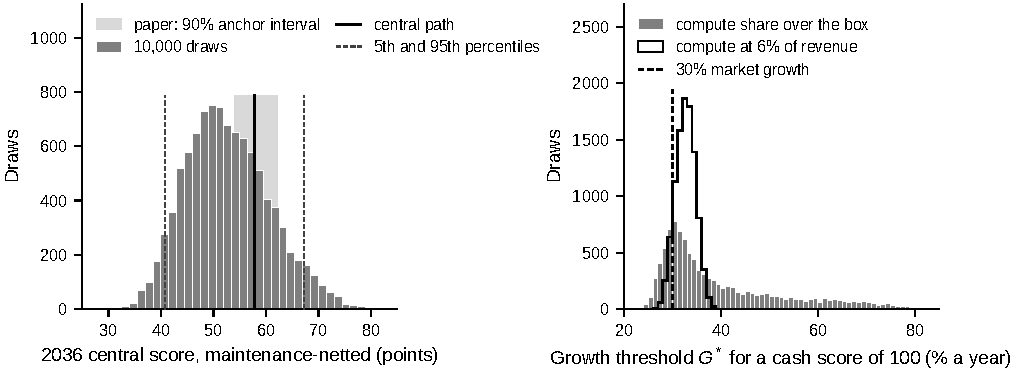
\includegraphics[width=\linewidth]{figures/fig_stress.pdf}
\caption{Joint-parameter stress test. Left: the central 2036 score on the netted basis over the \StDraws{} draws, against the paper's 90\% anchor-sampling interval; dashed lines mark the 5th and 95th percentiles of the draws. Right: the growth threshold $G^*$ for a cash score of 100, with the compute share over the box (\StCcBoxMin{} to \StCcBoxMax\% of revenue at 2025 prices) and at \CcCen\% of revenue. The draws are uniform on the stated ranges, log-uniform for compute per dollar of labor, an assumption, not a measured distribution}\label{fig:stress}
\end{figure}
